
\section*{}

\begin{minipage}[t]{.48\textwidth}
  \vspace{0pt}

\end{minipage}
\hfill
\begin{minipage}[t]{.48\textwidth}
  \begin{flushright}
    ``\emph{Du siehst, mein Sohn,\\
      zum Raum wird hier Zeit.}''
  \end{flushright}
  \flushright{\small{Richard Wagner, \emph{Parsifal}, act I}}
\end{minipage}
\vspace{1cm}


\section*{Introduction}
\label{sec:introduction}

\noindent
This chapter discusses the challenges and problems related to arts-based research (AbR) in and through non-visual arts, focusing on the use of virtual tools (interactivity) with specific reference to musical performance based on my own practice as an improvising musician. I believe that the needs put forward by this field, as well as several other real-time scenic and performing art forms, are not necessarily synchronous to those deployed by the non-real time arts.\footnote{It should however be noted that few art forms are unanimously non-real time or real-time. As far as time is concerned, music genres such as electro acoustic tape music---music produced electronically, recorded unto tape or disc and played back from the same---is conceptually close to non-real time art forms. Furthermore, the visual arts encompasses activities that that are highly dynamic and depend on real-time in ways similar to the ways music does traditionally.} Therefore the point of departure here is that research performed in the realm of the real-time arts, due to their peculiar relation to time and space (also beyond the more obvious ways), may differ from research performed within other art forms (also here beyond the more obvious ways in which these differences are deployed). The fact that in music \emph{action} takes place \emph{in} and \emph{through} real time rather than primarily \emph{over} time makes it an interesting, and equally difficult, candidate for artistic research. My primary interest, here and in general, is that which is commonly referred to as \emph{Interactive   music}; music where musicians interact with computers and other kinds of machines in real-time. 
The intricacy of the dynamics in the relationship between the man and the machine is of particular interest while working in the field of Interactive Music. But it is also a field that has a much wider scope considering the great challenges computer interface designers are facing and will face in the future as computers pave their way into new objects. The asimilarity in the way in which man and machine deal with time and memory in, is of particular interest, and may be understood from the point of view of a \emph{in-time} versus \emph{over-time} continuum.

In the following I will discuss real-time systems, i.e. systems that consist of a performer and a computer, in music, as well as in more general terms. The ways in which the questions relating to the object of research may be adressed will be discussed as well as how, and if, this object may be examined from the inside.
% suggesting a `field of the musical work' that may be examined from the inside.
After a brief discussion of time in more general terms I will turn to my own practice and use my experience from improvising on and with computers as a point of departure. The virtual, i.e. that which is offered by the computer, and the ways in which we may interact with it, is further brought into the discussion and the virtuality of the computer is compared to the virtuality of abstract artistic representation. The foundation for my position brought forward here is my experiences with working as a researching musician, composer and programmer in the realm of electro acoustic, and improvised musics. %Specifically, my artistic PhD dissertation ``Improvisation, Computers, and Interaction. Rethinking Human-Computer Interaction Through Music'' is used as a frame of reference throughout.

The aspect of interaction in the field of interactive art and media is problematic as the term \emph{interactive} to some extent has been hijacked by computer interface designers.\footnote{Susan Kozel similarly comments how the meaning of the word `virtual' is to be found when its ``overly reductive association with immersive technologies and that now anachronistic term cyberspace'' is removed.} Though one of its lexicographic meanings is ``Reciprocally active'',\footnote{``interactive, \textit{a}.'' The Oxford English Dictionary. 2nd ed. 1989. OED Online. Oxford University Press. 1 Nov. 2007. \url{http://dictionary.oed.com/cgi/entry/50118746}} its meaning in that context is more geared towards a methodology of control, than sharing, or mutual exchange. In the reduced meaning of computer interaction the actions of one part, `the user', is used to control the \emph{re}actions of the other, `the machine', often in a one-to-one relation: one action, one re-action, ignorant of prior actions and reactions. Musical interaction on the other hand is all about reciprocity, particularly in improvised music.\footcite[See for example][]{monson96} A successful interplay between musicians involved in an improvisation rests on a mutual sensitivity for taking, and responding to, musical initiatives. Musicians induce differences rather than alter states; they induce differences that ``\emph{make a difference}''.\footcite[And, according to Gregory Bateson, a difference that makes a difference is the definition of \emph{Information}][92]{Bateson} Even for an orchestra conductor---who is commonly seen as the \emph{director} of the music, commanding its flow---the agency of control is limitied to what can be achieved through interaction with the musicians in the orchestra. Interaction-as-control and interaction-as-difference are not clear cut definitions in binary opposition. Again we are dealing with a continuum; a continuum of interactive potential ranging from the most reduced form of interaction-as-control (click and response) to the infinitely complex interaction-as-difference (e.g. musical interaction). The activity of playing back a CD-recording of a symphony on a sound system is an example of the former while conducting a symphony orchestra playing the same symphony is an (extreme) example of latter. What one may gain in control with the CD player, the recording and the sound system---a CD can be paused, repeated, removed, etc.---we loose in influence over content. The CD recording will sound the same unless we destroy it, in which case it will not sound at all (only if we are lucky will we reach an intermediary stage where the CD plays back but the sound is deteriorated). As conductors however we may alter the music in ways that we see fit, limitied merely by cultural and social practices. But what we gain in influence in this context we loose in control: We can not as easily pause a live performance, considerable financial resources needs to be deployed in order to gather all the musicians needed, the training needed to be able to conduct a symphony orchestra is counted in years whereas the training needed to play back a CD is counted in seconds, etc.

Furthermore, when pushing the `play' button on the CD player, the quality of the physical movement needed to press down the button has no impact on the result. All that is needed for sound to be produced is that the threshold between on and off is surpassed. When conducting on the other hand, the nature of the movement has everything to do with the nature of the result. Conducting is an embodied activity whereas playing back a CD is not.

When the technology became useable in the early 90's, Virtual Reality was seen as a great potential for art production.\footcite[See for example]{moser96,wood98,dixon07} The virtual reality is a game of deception where there is no extension in space (although there appears to be one) and where existance depends entirely on the interactions of the subject with the virtual reality technology. The virtual is disembodied and it is furthermore truly non-ocular in its complete absence of a consented visual component. After all, that is one of its great qualities; the users are able to mold their own (virtual) visuality.\footcite[Compare to William Gibson's definition of Cyberspace as a ``consensual hallucination''][51]{gibson84} This visuality may be different each time. Or, it may be identical to any other visuality, since making duplicates is no problem in the digital realm of the virtual. As technolgy has advanced its positions in Western culture, the virtual is nearly ubiquitous. To define a virtual reality that is distinct from reality is almost not possible. There is a virtual aspect to almost all activities in the occidental World.\footnote{\cite[See][]{baudrillard02:screened}. I also write about the topic of the real versus the virtual in interactive music in \cite[ch. 4]{frisk08}}

The virtual world offered to us by modern technology is interesting from the point of view of Arts Based Research, both in the ways that it deviates from the real world, but also in the ways that it connects Art and art practice to aberrant practices such as Computer Science and Artificial Intelligence. Thanks to their ignorance of conventions and lack of long term memory and historical insights, machines are phenomenal individual forgetting devices.\footcite[See][]{miller04} The absence of an embodied relation between the machine and its operator is further consolidating the breach between human cultural heritage and the agnostic nature of the machine. In the virtual world nothing is hard wired, hence, muscular memory is useless: Any one physical movement can have a different meaning each time.\footnote{The synthesizer is the perfect example here: Though it looks like a piano keyboard, any key can produce any imaginable (machine) sound, and a different one each time, all depending on how the synthesizer engine is programmed. Hence, any physical, emobied knowledge a trained pianist has with regard to sound production is virtually useless while playing a synthesizer or a keyboard attached to a computer instrument.} Envision the four members of Kraftwerk,\footnote{See \url{http://kraftwerk.technopop.com.br/pictures\_80years.php} for some pictures from live concerts, in particular the image from the TV show `Na Sowas' from 1982 is significant.} standing still and expressionless in front of their keyboards (obviously exploiting this dissociate aspect of their relation to the machine-instrument). Compare this vision to the physicality of almost any acoustic instrument performer playing live in front of an audience. The lack of context particular to the virtuality of electronic music---an electronic instrument may be updated and revised after which integral aspects of it has been altered---is an asset, but it is also a great frustration to some.\footcite[E.g.][]{ostertag02} At best it enables novel aproaches to artistic problems or issues and at worst it creates expressions void of inter-musical (or inter-artistic) references. Aproaching this field as a researching musician is a difficult task and the scientific as well as the social and cultural aspects of the virtual should be taken into consideration. How can the (non-)spaces of the virtual be truthfully represented outside its own domain? How may it be documented and communicated in the context of AbR?


%In electronic music much of the research hitherto performed has had a strong connection to Natural Sciences that AbR should attempt to counterbalance. Not because there is an opposition in terms but because the 
 
%These questions become even more acute 

When dealing with real-time technologies in music these questions are again brought to the fore. The real-time `object', the music that is a result of real-time processes such as improvisation, live coding, interpretation, etc., is made up of a volatile substance that is not easily transformed to a researchable `object'. While investigating how the virtual sound worlds of computer instruments, created and edited in real-time, may interact with (or fail at interacting with) the real world, the questions pertaining to access and documentation will become important. 
%all of which are intimately linked to issues of time and space.
Although the Western tradition has developed powerful musicological methods to represent and document music visually,\footcite[See]{bregman94} independent of time, are there methods that retain the temporal identity of the object rather than do away with it? Such methods should also include questions rarely explored in AbR, such as the impact of contextuality and listener reception in musical and scenic performances. Also more multi disciplinary research projects will be of great interest here, in particular those that actively deal with visuality in different forms such as computer games and film. 
%considering the great impact video works has had on the electro acoustic music community over the last decade.

\section*{Time}
\label{sec:performing-time}

As stated above, performing music takes place \emph{in} time and I believe it is fair to assume that there is a difference between investigating `the object'\footnote{Let the object, for the moment, encompass all and any aspects of the artistic practice.} in-time, while it is unfolding, as opposed to doing it over-time, as a more or less static object. A researching musician needs to be able to explore the object in a multifaceted way, as a stratum of analytical modes in simultaneous operation. The question of time is significant as  
% but we will return to this aspect of it later.
%Whatever is performed, whatever is played, needs to be evaluated at the time it happens. 
many of the different processes involved simultaneously take place in  different time scales or temporal modes. While performing the musician measures the perceived sound against an inner vision of what was intended, and against prior performances, and the measuring is constantly performed at different temporal resolutions. Orchestra conductors are making judgements on the music in the present based on their knowledge and expectation of what will happen in the future of the music: in next bar, the next section, the next movement, the end of the concert, the next concert, etc. They are able to constantly keep a fisheye view on the piece without loosing the details in the process. The conductor is accessing the object at different rates and at different temporal locations, or points in history (and in the future), all at the same time. 

Electronic music composer Curtis Roads identifies nine different time scales in operation in the production and performance of music ranging from \emph{Infinite} to \emph{Infinitesimal}.\footcite[][ch. 1]{roads} The former is the time span of ideal mathematical durations such as the Fourier transform with its infinite series of sine waves,\footnote{A Fourier transform, named after the French 19th century mathematician Joesph Fourier, calculates the frequency spectrum of a sound by describing it as the sum of an infintie series of sine a cosine waves.} and the latter is the equally ideal time span of mathematical durations such as the delta function which represents infinitely brief intervals of time. In between these two extremes we find the Supra, Macro, Meso, Sound object, Micro, Sample and Subsample time scales. An interesting remark made by Roads is that the discontinuities that appear in the boundaries between the different time scales gives rise to perceptual differences in sonic events.\footcite[4]{roads}  A note terribly out of tune in one temporal order may have just the right intonation in another, and a beat out of sync in one time scale may swing in another.\footcite[For an example of the great variation in rhythmic timing among jazz musicians when observed at high temporal resolution, see][]{friberg02} 

To the Greek composer and architecht Iannis Xenakis the discontinuity of time was of pivotal import. Not only the interruptions that occur when moving across the boundaries between different temporal scales, but also the separability of events occuring within the flux of one particular time scale. According to Xenakis, non-synchronicity and discontinuity of events in time is what makes the flux of time perceptible: Without it time would remain hidden, illegable and inapproachable. Painting a picture of chains of events that makes time come forward, Xenakis also argues that their representation in the brain---our memory of events in time---is a generalization and abstraction that exists outside of time: ``Memory is the spatial translation of temporal (causal) chains.''\footcite[263]{xenakis71} 
Contiguous events, separate in time, creates durations in the flux of time and marks out spatial distances in its memory representation: Time becomes space. Following this line of thought, music is an art form that, in most cases, participates in space as part of a temporal flux. It lays out events in the flow of time, a flow which in itself, in some cases, is controlled by these events. But, according to Xenakis, at the same time, the same music, also exist outside of time as a snapshot, as an abstract representation.
This representation, when encoded in our memories, or when described as a musical structure (e.g. a fugue), becomes accessible to us as a whole. A whole which we can navigate, jump back and forth in, and sustain at random access. The whole becomes, not a succession, but something non-temporal that ``can be viewed as one \emph{time spectrum} of a fundamental duration''.\footnote{\cite[73, my italics.]{roads} See also \cite{stockhausen57}}
That in-time processes such as music are transformed to images or gets spatialized in the human brain is a common thought, but the fact that Xenakis uses the idea of a time \emph{spectrum} is interesting. When the frequency spectrum of a sound is calculated using a Fourier Transform, increasing the resolution in frequency reduces the temporal resolution, and vice versa. It is not easily possible to simultaneously retain high frequency resolution \emph{and} high temporal resolution. In the time spectrum that Xenakis is talking about, a whole in which an entire compositional structure is encoded, there is a similar trade-off between temporal resolution and spectral resolution. Returning to his claim that memory is a spatial translation of contiguous events in time: Perhaps it is to be seen as a spatial spectrum of a fundamental duration, a way to look at the structure as a function of space rather than a function of time. The time spectrum---which should really be called a \emph{space} spectrum---transforms events in time to events in space, and the reverse transforms spatial properties in events to temporal properties.

Perhaps Xenakis' idea of a musical memory as a spatial translation of the musical events contained in it should be traced to his background as an architect, and is influenced by his aptitude and sensibility for spatial rendering. If we limit ourselves to the realm of the time based arts, is it really possible that our in memory representation of something such as music, that exists and evolves in time, can be represented independent of time? And if it is, what is the coupling between time and space that makes the transformations from one to the other transparent; how is the space/time spectrum calculated? These are examples of questions that may be tackled from within an artistic practice in the context of AbR. Only from within the flow of time is it possible to fully grasp the time-space transformations and their significances, specifically as well as generally. Furthermore, the results of such an interrogation performed from within, are likely to be different from those obtained from the outside, and hence they have the potential to contribute new knowledge to several fields if inquiry.

To briefly return to the concept of musical events outside of time and the whole as a time spectrum, it should be noted that the idea of timelessness exists also from within the musical flow. Timelessness in music is commonly coupled with minimalist music or indeterministic expressions such as those by John Cage\footnote{See for example John \citeauthor{cage62:atlas}'s \citetitle{cage62:atlas}for which Cage used a star atlas to generate the pitches and amplitudes for the score (\cite{cage62:atlas}).} where succession and causality, harmonic or otherwise, is made unimportant. To experience such music can in some cases invoke a sensation of timelessness, despite the fact that the listener is in the midst of the flow of time, of singular events in a discontinuous stream. According to musicologist Jonathan D. \citeauthor{kramer88} this kind of vertical expression ``is a holistic music that offers a timeless temporal continuum, in which the linear interrelationships between past, present and future are suspended.''\footcite{kramer88} It resists linear reasoning. But temporal verticality is not only to be found in music. \citeauthor{kramer88} mentions Samuel Beckett as an example of an author (among others) that resists the Aristotelian dramaturgic succession with the purpose of extending the present, the now.
Frederic Rzewski's composition \emph{Les Moutons de Panurge} is an example of timeless music, a piece that employs vertical time. It sets up a state and stays within it. It tries not to establish time and sucession but it tries to elongate the present. What then is it that evokes the sensation of timelessness the listener may experience while listening to a piece of vertical music? And is it connected to Xenakis's time spectrum, a representation of time outside of time?

Timelessness cannot simply be the absence of time; the expression (or impression) of timelessness cannot be the negation of the time it fails to manifest. On the contrary, turning to J.T.\citeauthor{fraser90}'s  book \citetitle{fraser90}, \citeauthor{kramer88} proposes that it is the multiplicity of facets of time simultaneously present in the mental and physical reality of every human being that makes possible for certain pieces to evoke the sensation of timelessness. Atemporality---one of \citeauthor{fraser90}'s temporal horizons---is only one temporal mode out of several possible (the others being Protemporality, Eotemporality, Biotemporality, Nootemporality, Sociotemporality). A given piece of music may resonate particularly well with one temporal mood and will thereby shadow the others. If Rzewski's music evoke timelessness in the listener it does so because the atemporal \emph{Umwelt} of the listener overshadows the other, perhaps more linear and flowing temporal modes.

There are several important aspects for the current discussion in this reasoning of which the first is the concept of a multiplicity of temporal modi. Many different time scales are active, influential and operative simultaneously and it is possible, for the listener as well as for the performer, to move between them. Although it is also true that this movement alters the listeners perceptions, the moving between timescales and the coexistance of multiple timescales is also possible without the discontinuity brought up by \citeauthor{roads} and discussed above. The second interesting aspect is the fact that \citeauthor{fraser90} does \emph{not} define atemporality as a negation of time. It is a temporality in which succession is an impossibility, where the only temporal relationship is simultaneity, but it is still a temporality among other temporalities. No tranformation to a spatial representation is made. This suggests that, in place of the `in time' or `outside of time' dichotomy along with the transformative operations involved when moving from one to the other, we may find a multiplicity of temporal layers coexisting and that we are able to continously move between these layers. 

%This is an important fact that has an impact on the discussion when we move from abstract theory to practice.

But before engaging in the practice of the improvising or interpretating musician we shall return to the in-time versus over-time distinction. This distinction is obviously interesting with regard to the topic of time and temporality, but it is also of interest to the specific topic of Interactive music. As a genre, Interactive music descend from Computer Music, also called Electro-acoustic music, and has strong interdisciplinary connections with subject areas such as Artificial Intelligence, Cognitive Science and Computer Science.\footcite[24]{moore90} These disciplines are concerned with trying to understand human behaviour and, to some extent, attempt to mimic that behaviour in machines. In the context of AbR it is obviously important to draw upon knowledge that emanates from related fields of inquiry but it is equally important to re-evaluate those same sources. Historically there may have been a tendency for Computer music to lean against the natural sciences that, in fact, may also have much to gain from learning from the artistic practice of Computer music. The concept of time in general and the in-time aspect of music in particular.

%All of these disciplines share a wish to understand 
% due to its origin in cognitive science and, more specifically, robotics. Both of these fields are concerned with making machines imitate or mimic human behaviour, the former in the shape of musical expression.

\section*{Performing in practice}
\label{sec:performing-practice}

The distinction between activities that take place \emph{in} time and those that takes place \emph{over} time is brought forward in a short report by cognitive scientist Tim \citeauthor{smithers96}.\footnote{I am indebted this reference to Vijay Iyer who is referring to it in a discussion on embodiement in improvisation. See \cite{iyer08} For the original source along with a few additional on the topic of robotics and cognitive science, see \cite[See][]{smithers96,vangelder98,smithers:98}} Actions that take place in time are actions where the time taken matters, where time is a factor whose value is decisive. For example, when I walk it is not just that my leg is moving that matters but also the time it takes to move it. As for actions that occur over time, the time consumed by the action is of little significance for the result. Computation is a typical example of an over-time operation: The primary interest is the result itself, and as such it will not be affected by the amount of time it takes to arrive at it. Much (but not all) of art production, at least in its early stages, are over-time activities as well as most other abstract operations. Painting a picture, conceptualizing an art installation or writing a musical score are over-time operations even if the result, or the instantiation of these art works are in-time operations. Musical performance and improvisation are typical in-time operations: They are \emph{embedded in time} (to use \citeauthor{smithers96} expression) whereas over-time operations may be said to be \emph{contained in time}. Along with advances in computer science and robotics, real time computation has altered the picture somewhat, but the difference between an over-time operation being so fast that time goes unnoticed is very different from the way the mind ``exploits both the constraints and allowances of the natural timescales of the body and the brain as a total physical system.''\footcite[276]{iyer08}

%Its physicality and the relative speed---relative to a multitude of factors---of the events. 
% a characteristic of great importance in the context of Arts based Research: 
%But in that case, how can such an activity at all be (re)represented and make up a researchable object if it cannot be abstracted and resolved of its temporal prison? 
%How can such an object be successfully researched from the inside?
%Without attempting to fully disentangle these questions here I will merely suggest that 
%In other words, research from within time based arts is indeed possible. 

Something that is embedded in time will always be difficult---but not impossible--to conceive of as an object (though object is a misleading term here) independent of its temporal context. This `object' will not easily transform itself to a spatial representation along the lines of what was discussed above, because it is not just the order of events and the speed at which they are deployed that matters and that gives this object its character. The performer/researcher working in the field of AbR should resist the temptation of objectifying the in-time performance and instead embrace the possibilities and the great challenges that lies in investigating the in-the-moment, unfolding, real-time, processes of creative and interactive activities. These depend on properties that will not transform themselves to out-of-time representations without something substantial being lost. Their in-time aspects, such as their physicality, and intersubjectivity, are primarily accessible from the inside, from within the creative activity. They will risk at loosing their identity if resolved of their `in-timeness', if they are instead looked upon as over-time processes but it should be noted that attempting at such research is a difficult endeavour. I will argue that for AbR in time based arts to be different from e.g. standard musicological research, it has to face these difficulties and attempt at accessing the object form the inside and research the in-time object as it is unfolding. The means to do it and the methods to use will inevitebly have to differ from case to case and from discipline to discipline but investigating and acknowledging the difference between divergent temporal domains and temporalities is a common prerequisite, regardless of the discipline. In other words, to engage in AbR, accessing the object of research as an in-time process constitutes an actvity that may offer an interesting aternative to the otherwise dominating visual modes of research expressions. Discussing the practice of an improvising musician without resorting (solely) on transcriptions of the performances, or other abstract representations, is likely to render a result different from traditional research, or AbR that primarily takes place outside the temopral flow of the object. To visualize a flow of time, i.e. to perform the kind of time spectrum transformation as was suggested by Xenakis above, is admittedly a powerful and pedagogical conjuration\footnote{A popular example is the famous scene in Hitchcock's 1959 movie \citetitle{hitchcock59}. Madeleine (played by Kim Novak), whose identity is overwhelmed by her great grand-mother, is standing in front of a cross section of an over 1000 years old Redwood tree. She places her finger towards the outer ring of the tree and marks out the point where she was born and the point where she died. The distance between the two points is short relative to the size of the tree, and, as she is moving her finger across the wood, she says ``It was only a moment to you''. \cite{hitchcock59} The cross section of the tree is used to spatialize a (short) life span, to transform a duration to a distance, to transform time to space. Another, similarly schizophrenic, example is the end of the first act of Richard Wagner's opera Parsifal (cited above) where there is a slightly more subtle and continuous transformation from time to space. Parsifal makes a remark that, despite his slow pace he already seem to have come far. The explanation offered to him is that ``time here becomes space''. \cite[See][act 1]{wagner82}} but it is equally deceptive: It is a transformation of an in-time process to an over-time process, and in the shift, temporal as well as other kinds of information is bound to get lost.
%It is perhaps possible to argue that it is the responsibility of AbR in real-time art forms to access the object from within the process as this is not possible in other means of research. In the context of AbR the in-time aspect of musical performance and other real-time art forms should not be seen as an hindrance, but as a great asset 


\begin{figure}[htb]
  \centering
  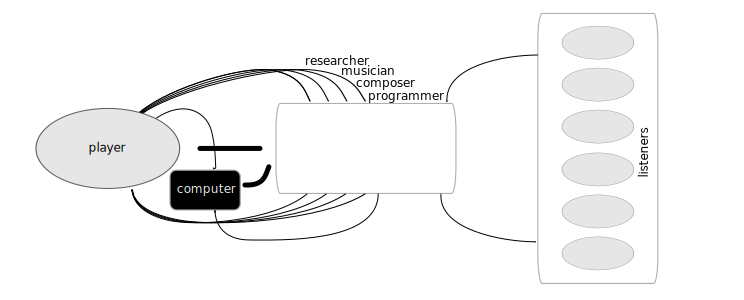
\includegraphics[width=\linewidth]{img/player-computer}
  \caption{\small{A simplified graphic representation of an instant of an improvised performance with an interactive computer. The performer is reflecting upon the output in several different modes of thinking (represented by the arrows leading from the preformer to the sound). The feedback of the reflection and its influence on the object is represented by the arrows leading from the object back to the performer.}}
  \label{fig:player-comp}
\end{figure}

As a performer, engaged in an actual performance, and simultaneously a researcher, I obviously combine several different roles and disseminating processes at once. As can be drawn from the graphic in Figure \ref{fig:player-comp} I at once access and evaluate the object in different modes of thinking relating to the different tasks I carry out or have carried out in preparation for the performance (programmer, musician, composer, etc.). The object in this case is simplified to constitute the bare audible (poietic) trace left by what I and the computer produce together. Similar to how it was noted with regard to the conductor above, the evaluation is simultaneously done at different rates and against different templates, expectations or value judgements (of which some may be upright banal): Is this note in tune? Is this good music? Does this work against the pre-conceived form? Is this computer program functioning the way it should? Will this work in the next concert? 

Apart from the performance specific reflections there is the additional layer, particular to AbR, of the research activity. In my own experience as a researching musician/composer the point of intersection, the convergence, between the in-time music and the research upon that process, is an area laborious to navigate wisely and honestly. It is easy to get lost and it is easy to get drawn outside of the temporal flux so particular to the musical practice. It is always tempting to detach the researcher from the in-time process and let the research operate in its own temporal mode, more closely related to how musicological activities are carried out. Intimidating questions relating to the validity of a research performed from within \emph{bad} art (i.e. bad art but good research) makes the task even more difficult for the researcher. (No artist researcher will be proud to have performed excellent research but bad art.) However, many of these distracting questions relate to the (false) idea that the researcher could somehow be discrete from the musician, as if a Cartesian split between the rational investigator and the unpredictable creator was possible and desirable. 

\begin{figure}[htb]
  \centering
  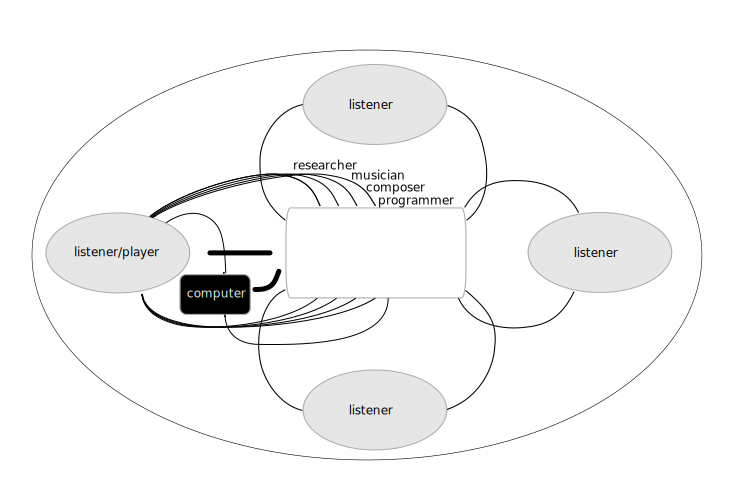
\includegraphics[width=\linewidth]{img/player-listener-computer}
  \caption{\small{A modified version of the previous graph (see Figure \ref{fig:player-comp}) where the listeners and the performer are united in the act of listening. A linear conception of a producer and a group of consumers is reduced in favour of a distributed sphere of listening.}}
  \label{fig:player-comp}
\end{figure}

In the graph representing a slice of time of a performance (see Figure \ref{fig:player-comp}), the trajectories of reflection create a feedback loop between the object of research and the musician. A corresponding loop may be found in between the listeners and the music representing the listener's reflections upon the music as it takes place in real time. Although not likely to be entirely synchronous with those of the performer, provided the performer and the listeners share some musical references or have a common cultural ground, it is conceivable that some of the reflections made by the listeners overlap with some of the performer's. If I choose to play a note out of tune it is only if the significance of the `out-of-tuneness' is obvious to the listeners that they will appreciate it as something that adds to the music. If the significance of the pitch alteration is beyond reach it is more likely they will hear it as an error that maybe even reduces the value of the performance. It is as a listener I (as a performer) am able to reflect on that which I play---In a wider sense I am first a listener and then a performer since everything I play is a result of what I hear or have heard. Hence, the audible trace produced by me is an object for reflection common to both myself and the listener, a suggestion that would resolve the producer-consumer conception in favour of an intersubjective relation. Marcel \citeauthor{cobussen08}, in his book \citetitle{cobussen08}, discusses listening and suggests an understanding of ``listening to music'' that really means ``listening \emph{to and fro} music''.\footcite[p. 135 (italics by the author)]{cobussen08} When experienced, this oscillating movement of coming and going moves beyond the the idea of the listening subject and the sounding object. According to \citeauthor{cobussen08}, ``to listen to and fro decenters them, wipes them out.''\footcite[135]{cobussen08} Through the shared act of listening the subject-object divide between the listener and the sounding object is erased, and the producer-consumer distinction between the performer and the listener is blurred. 
%Would it not be fair then, to suggest that the shared listening activity between performer and listener similarily decenters the creator-listener distinction? We have two 
If the performer is a listener among other listeners, the traditional flow of communication from a (non-listening?) creator to a listening subject becomes difficult to maintain. Instead we are presented with the image of a group of listeners in which some members are \emph{also} performers and creators (see Figure \ref{fig:player-comp}. I am not a performer that listens, I am a listener among other listeners that also performs. According to Vijay \citeauthor{iyer08} the sense of ``shared time'' is a property of music listening and is a crucial aspect of the temporality of performance. Listening to a performance of improvised music is to experience the improvisers real-time struggles, their in-time processes. Also to non-dance oriented music, listening to music is a co-performance, a ``participatory act of marking musical time with rhythmic bodily activity [which] physicalizes the sense of shared time, and could be viewed as embodied listening.''\footcite[276]{iyer08} 

In the feedback loops between the performer and the audible trace it is difficult to separate artistic evaluations and reflections from those that are research oriented. Or, perhaps more accurately described, also a research oriented reflection may very well result in an alteration of the object, an alteration that changes the music. The research activity may further constitute meta-reflection upon purely musical reflections, i.e. reflections upon reflections (\emph{Why is it important that this note is in tune?}), but that does not prevent them from induce change in the music. In other words, although the trajectories of reflection may be distinct from one another, their responses are not. This is particularly obvious in Interactive music. If an interactive scheme is deviced that will trigger a response upon a certain stimuli, if the desired response is not achieved, i.e. if the interaction fails for some reason, it will obviously affect the music. Not only because the desired response did not trigger but maybe the performer will make the triggering phrase louder, slower, shorter or faster; anything in order to facilitate recognition for the computer. A reflection upon past and current events in one domain (\emph{the computer missed my cue}), induces a change in another which in turn may lead to altered decisions in yet a third domain.

The computer, located to the right of the performer in the graph, is clearly of significance to the discussion here. One way of working with Interactive music is to use the computer as a commentator to what is played. A commentator that may have its own agenda, its own musical material, but which depends on its musical input so much that it is not able to produce sound unless live input is given to it. The computer program may have pre-conceived structures that stimulate certain responses from a co-performer. Writing such a program is an over-time process, not unlike composition. A performance is imagined and functions are implemented. These functions may, for example, resonate with a particular kind of timbre, which, in performance will influence in-time decisions. 
Writing a composition and performing it involves similar kinds of tensions between over-time and in-time decisions but the interesting aspect of the interactive computer is that whatever the agenda used to construct the program, if the interaction is successfully exploited, the agenda may be altered not only in the performance but \emph{by} the performance. A musical score on the other hand, is not easily changed during a performance.\footnote{To be fair, any performed composition is altered by its performance in one way or another, but, in the Western art music tradition, radical in performance alterations of the written music are more likely to be called mistakes rather than interpretation.}  

The in-time reflection of the output of the computer and of the interaction with it can relate to many different aspects of a musician-computer system. It may be a reflection on the in-time musical output of the computer (the sounds it is producing), on the over-time abstract functionality of it (its algorithms and basic processes), or to some in-time but non-musical process it performs (e.g. processing data from sensors). Or, it can be a combination of these and other modes of reflection. Without a doubt is this one of the more challenging aspects of being a computer musician: Having to evaluate abstract functionality of a computer program in performance easily disrupts or distorts the temporal flux of the in-time process of the music. The musical in-time evaluation of a series of events emanating from the computer, made without knowledge of, or interest in their origin (i.e. the musician's particular interaction with the computer), will not necessarily correspond to an evaluation of the same events from \emph{within} the process. The consequence may be that, in a response to the performer's reflection, a change is introduced in the output that, to a listener, who is primarily concerned with the audible trace, and may be unaware or unconcerned with the details of the musician-computer interaction, sounds awkward. The differing modalities of reflection which have their roots in differing temporalitites, creates a breach between the listener and the performer. The temporal differences is one aspect of the issue at stake here, but it is not the only one. 
%However, the virtual aspect of the computer is likely to be another. 
Due to a poor performance, bad programming or some other factor the virtuality of the computer instrument fails to reveal itself and the musical decisions made by the performer becomes enigmatic to the listener.
Either way, the use of the computer in live performance shows that in-time and over-time processes are not mutually exclusive. They can co-exist but their zones of interaction may also result in noise and a distorted perception. To hold different temporal representations active at the same time may be second nature for a musician, but the added aspect of the interactive computer makes it both more complex to understand and more difficult to perform.

% Xenakis claims that ``one could say that every temporal schema, % pre-conceived or post-conceived, is a representation outside time of % the temporal flux in which the phenomena, the entities, are % inscribed''.\footcite{xenakis71} If the programming of the computer % represents such pre-conceived temporal schema and I am able to access % it, make use of it and, interact with it in an improvised performance, % I would conversely argue that such schemas are \emph{not} % representations out of time. They contain time
%The virtual world of the computer 


% But the opposite is also possible: It may create a change that, due to % its originality, has a positive influence. There are two points to be % made here: i. In-time and over-time processes are not mutually % exlusive. ii. When the occur, in parallel as conscious processes, one % may distort the other.







% The cone becomes a valid metaphor for understanding the strata of time % scales present in the mind of the performer at the time of % performance. The ability to leap back and forth between the present, % the past and the whole (the current performance in its history and % what is yet to come) is significnt to the practice of a musical % performer. The whole in this case becomes not a succession but ``can % be viewed as one time spectrum of a fundamental % duration.''\footnote{\cite[73]{roads} See also \cite{stockhausen57}}


\section*{Interacting with the Virtual}
\label{sec:inter-with-virt}

The almost mystical sensation of simultaneously being able to be in time, `now' and in memory, in the recollection of a previous now, is an important and powerful aspect of time-based arts in general and music in particular. Imagine listening to a well known melody being played. As the melody is unfolding there is a perpetual interaction between its in-memory representation and its real-time representation. Sometimes, if the memory of a particular music is really strong, it may overshadow the real life version of it and inversely, if the performance is powerful and expressive it may smear out the original memory, overwriting it with the new version. As was discussed above, tt is tempting, and practical, to gather musical events into larger structures (e.g. notes into melodies, movements into symphonies, songs into songcycles, etc.) and regard them as singularities, as image representations of what they represent. As such they would have no reference to time, their temporality gets transformed to a kind of spatiality. Conceptually they would approach the ideal mathematical formula and become a representation of what  \citeauthor{roads} refer to as \emph{infinite time}, or, to put it in Xenakis' words, time is abolished in such structures: ``[O]ne could say that every temporal schema, pre-conceived or post-conceived, is a representation outside time of the temporal flux in which the phenomena, the entities, are  inscribed''.\footcite[264]{xenakis71} They become spatial, and virtual, translations of the original in-time representations. From a research point of view it is of great interest to understand if it is true, as Xenakis claims, that time really is abolished. And, if it is, how is is that we can keep track of such time specific data as duration, and silence, in memory representations of music? The question is not merely of theoretical or philosophical import, it has great impact on the way we understand and execute Practice based Research in the real-time arts. To examine a musical practice from within---as opposed to examining it from the outside---we need to be able to access the object in real-time. And to gain access to it in real-time it is necessary to understand what real-time is relative to non real-time, i.e. in-memory representations.

In the survey of memory and imagination in Paul Ric{\oe}ur's seminal book \citetitle{ricoeur04} among many other things in the first chapter, he critically discusses Husserl's concept of memory in general and the ideas of \emph{retention} in particular.\footnote{The full meaning of this concept and the significance of Ric{\oe}ur's thinking upon it is far beyond the scope of this chapter. I use these sources as inspiration and I do not intend to unwrap a full philosophical discussion on time.} The duration of a musical note is used to address the question of what it means for something that endures to remain. And this is indeed at the heart of the matter for the present discussion: When in music, or any other real-time art form, we perform there is a complex interplay between creation and duration. Musicians do not only play series of intances that are sequentially combined, they play notes, phrases and gestures that have a duration. These entities can be acessed by the performer as a series of instants, or sub-entities, but also as a unity, a whole, that may signify something far beyond the sum of its parts. Something which has both a virtual, in memory, and a real representation. These entities endure and as they develop in time, they create duration.

How is this possible? How can the present `now' and the memory of the past `nows' coexist? How can the memory of the preceding now co-exist with the memory of a now six months ago? Husserl, with the sounding note as an example, states that a musical note as it is played makes the now perceptible, and, as it continues to sound it ``has an ever new now, and the now that immediately preceds it changes into a past.''\footcite[\emph{Vorlesungen zur Phänomenologi des inneren Zeitbewussteins}, Husserl, E. cited in][32]{ricoeur04} The `ever new now' is what constitutes the modification in the perception that constructs the duration. The `now' that is pushed back by the `new' now however is not dissapearing but is held on to, and it is this `holding on to' that Husserl labels \emph{retention}.\footcite[32]{ricoeur04} Hence retention is, in a manner of speaking, a way to hold on to the note while it is sounding. It is not its memory, or recollection, but its modified perception. Neither is retention and imagination the same thing. And although the retention of a note and its present `now' are not the same thing, together they constitute the experience of the note as a whole, as a duration. But as long as the retention lasts ``the tone has its own temporality''. Retention is a modification of perception and the difference between them is first and foremost a temporal one. Perhaps it is possible to imagine an interaction between retention and  recollection. While holding past `nows' of that which is unfolding in time in retention one can simultaneously recollect previous instances of the same expression (a note, a phrase, a gesture, etc) and compare the two. While the `now' continuously begins and recedes, with past nows sinking into retention, recollections rise from below and create a virtual now parallel to the real now. A new now that can never become the `real' but one which can trail the present. It can be experienced almost as if it took place in the real domain. A virtual (re-)presentation moving alongside of, or being pulled by, the real in a continuouos flow in time.

For a musician the real and the virtual as sketched above are two modes of listening: Inwards, listening to past experiences or outwards, listening to one's own or others' sounds as they disclose in time. In practice the musician can not fall back on only one of these modes but must let both the real and the virtual listening co-exist. ``The virtual is the invisible'' as Susan Kozel writes but not as ``raw potentiality'' as much as a hidden parallelity. Furthermore, this virutality is different from, but loosely related to, the virtuality of the computer and its interactive potential. 

According to Henri Bergson we can look at the present-past axis as an inverted cone (think an icecream cone) where the tip is the present and the base represents the oldest unconscious memories. Each segment of this cone, where a segment is a line trisecting it somewhere between its point and its base, represents a virtual plane, a region in the past.\footcite[][Ch.3]{bergson91} 
%Deleuze writes about these regions of the past as virtual sections 
In Gilles Deleuze's reading of Bergson each such region contains the totality of the past in different levels of contraction or relaxation and at any time we can make a leap to any segment of the cone, to any past memory, bringing it back into consciousness.\footcite[][60]{deleuze88} The cone is not to be understood as a storage device in which memories are put, slice by slice in succession, but rather it is an abstract visualisation of the human capacity to place oneself in the past, while still having access to everything prior to that particular point in time, as well as everything past it: ``It is in this sense that one can speak of the regions of Being itself, the ontological regions of the past `in general', all coexisting, all repeating one another.''\footcite[61]{deleuze88}
The cone symbolizes a dynamic process, more dynamic than what the image can represent, for there are several motions in simultaneous operation. The tip of the cone, which at all times represents the present moves perpetually along the plane of existance, ``of my actual representation of the universe'' all while the base of the cone remains still. If this is the horizontal movement there are corresponding vertical movements where pure memories are descending down to the tip, to where action takes place, and images from the present are ascending up into memory.\footcite[See also][47-8]{lawlor03} In other words, we have two contrasting movements, one of the cone moving on the plane and one inside the cone affecting the level of contraction at any virtual plane within the cone. Hence the virtual plane of memory is not a static \emph{image} (space) of a time in the past (a sound), but a constantly changing one. Following this conceptualization of the relation between the present and the past, the idea of a temporal schema outside of time that Xenakis brought forth should perhaps be questioned. In my own experience as a performer, the memory of a musical event vividly holds on to the temporal aspect of its origin. My memory of it is a memory, not outside of time, because the temporal relations between the events contained in it matters to the actual memory.

\begin{figure}[htb]
  \centering
  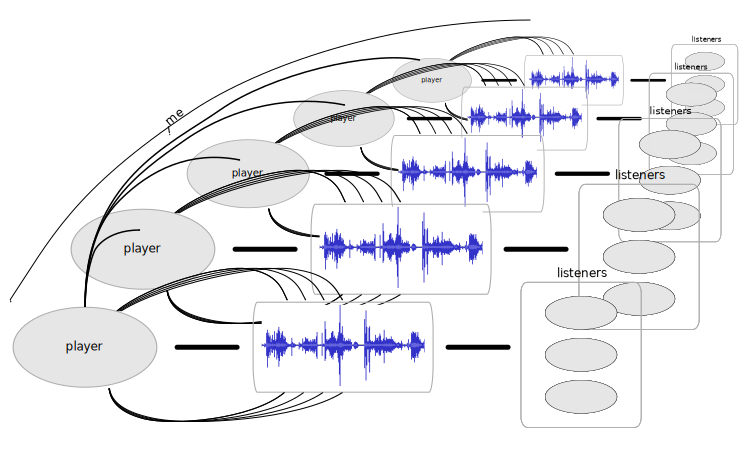
\includegraphics[width=\linewidth]{img/players-perspective}
  \caption{The imaginary performance as sketched in Figure \ref{fig:player-comp} with the addition of time. Past events are fading out but held on to by the in-time performer as is represented by the arrows pointing back unto previous nows. It should be noted that this is a extremely simplified graphic representation of phenomena that are infinitely more complex.}
  \label{fig:u}
\end{figure}

These virtual planes of memory are likely to be linked to the virtuality present in all musical creation. Common to both the virtual planes of memory and to the virtuality of music is that, although they generate visual elements and images, they do not depend on them.
But in real-time performance, in improvisation---in the spur of the moment---the leap from `now' to a virtual plane of the past may create a breach similar to how musical decisions made based on information hidden from the listener creates a breach, as was discussed above. An ontological difference that, in the best case, fuels a musical performance and takes it to new heights, but at its worst, detaches the performance from the logic of the `now', and the virtual plane fails to actualize itself and remains trapped in the memory of the performer(s). These leaps may be carried out as a result of affectivity within the performer or simply by aesthetic choices.

In Figure \ref{fig:u} the slice of time discussed earlier is now put into the context of the flow of time. Past events are slowly sinking into retention but the reflective listener-performer is able to make a leap back in time. Although only the activities of the performer are plotted, similar leaps back in time are obviously also performed by any given listener.

% \section*{Art practices and temporality}
% \label{sec:visu-arts-temp}

\section*{Summary}
\label{sec:summary}

``Composition liberates time so that it can be lived, not stockpiled.''\footcite[][145]{attali85}

The distinction between in-time processes and over-time processe in Art is obviously not clear cut. As has already been pointed out most artistic practice are over-time processes, at least in their initial stages. One exception is the improvisatory practices, particularly in music and theater. Improvisation depends extensively on its in-time processes. Group improvisation is a good example of how the allowances and resitances of the participants are part of, and affects, the in-time flow. However, even when engaged in an improvisation, the performer is bound to resort to over-time acticity such as leaping back into memory or making in-time choices based on over-time aesthetic judgments, also involving leaps.. In that case, what, if any, is the difference between the real-time artistic practices and other artistic endeavour in general and time-based artistic practice such as Performance art and Video art specifically? Perhaps the difference is mainly ontological.

We have seen that, using technology in live performance may disrupt the in-time process in varioous ways. In his book \citetitle{dixon07} Steve Dixon discusses the problematic issue of `liveness' in performance. There is a common sense that technology have ``transformed or destabilized notions of liveness, presence, and the `real''',\footcite[127]{dixon07} suggesting that the real-time arts somehow becomes less `live' when technology is made use of. Similar ideas have been discussed in this chapter based on the notion that it is the temporality of technology that is different from the temporalities of live performance. At the same time, even without technology, a performer and its audience simultaneously employs a number of different temopralities. Hence, the multi-temporality experienced is not a property specific to performances with a virtual component, but is common to much of performance practice and listening.

Art practice categories are to a great extent overlapping and there are sub-groupings within the larger containers of `Visual arts' and `Performing arts' that appear to be more closely related. Video art and Sound art, are two practices that have much in common with any Performing arts practice, in particular sound art, which commonly include works of composers such as John Cage and LaMonte Young.\footcite[See][]{labelle06} The works of these two composers and those of many other contemporary sound artists, are in every respect conceptually similar to any other musical work \emph{not} categorized as sound art. The difference, one may assume, is primarily ontological. Because Sound art belongs to the Visual arts it may be more likely to be considered as an over-time process, one that may be stopped and restarted and randomly accessed. One that lives outside of the flux of time and whose aesthetic criterias are independent of its in-time properties. Now, it should be made clear that in the Western music history there is a similar tendency of disregarding the performative aspects of a musical work and regarding the score, i.e. its graphical representation, as equal to the identity of the work.\footnote{The topic is brought up by British improviser and composer Trevor Wishart who asks what constitutes music: ``what we experience in the sounds, or what we might theoretically appreciate of the score through the sounds [\ldots].''} The ontolgy of the musical work is a topic beyond the scope of this chapter but suffice it to say that there is a similiarity in conception between a musical score as an independant, out-of-time representation and the non real-time arts
including some cases of sound art.

Alvin Lucier's seminal \emph{I'm Sitting in a Room} \footcite{lucier69,evens05,labelle06} is an example of a piece of sound and performance art. The short instructions for the piece tells the performer to read a written text into a microphone, recording it unto a tape recorder. The recording is played back and the sound, as heard through the speakers, is re-recorded unto another tape recorder. The process is repeated until the voice has completely deteriorated and only the resonances of the room are heard. In its live version, this piece makes use of all possible different temporalities and virtualities. As such it exemplifies not only a cross over between art practicies, it also shows that the specificity of the real-time arts may also belong to expressions more closely related to the non real-time arts.

Although there may be an ontological difference between works emmanating from the Visual arts and the Performing arts, a given work in either one of the two categories may be analyzed and investigated as a real-time performance. An art-work temporality is not primarily tied to its genre but is a result of the ambitions of the artist. From the point of view of AbR, any results gained from an investigation performed from within a Video work, from within a work of Sound art, or from within a Performance work will obviously be of equal interest. However a  difference may be acknowledged between works in which the real-time properties in themselves have an onotlogical importance with regard to the art work, and works whose representation rests primarily on out-of-time preperties and over-time processes.


Throughout this chapter I have tried to show how the real-time arts, with a specific reference to real-time Interactive music, depend on the in-time aspects of the processes they set in motion. Although music has had an out-of-time representation ever since musical notation was introduced, with the advent of recording technology sound, through the engravings on an LP or the holes in a CD, was transformed into space.\footcite[``We might say that recording is a reflux, or distillation in which time is boiled off, for time must be added back in to get sound, in the form of a steady motion of the turntable or tape heads or the crystal clock in digital recording.''][54]{evens05} And in this transformation, music was commodified. But with the spatialisation of sound came also the possibility for an unprecedented temporal precision.\footcite[4]{moore90} A precision which allowed for the study of sound, for microsound,\footcite{roads} and for scientific repeatability. To relocate the stockpiled, spatialized sound from its over-time representations to its in-time representation and perform the study of it in that domain, is one of the great challenges of AbR. 




%%%%%%%%%%%%%%%%%%%%%%%%%%%%%%%%%%%%%%%%%%%%%%%%%%
%%%%%%%%%%%%%%%%%%%%%%%%%%%%%%%%%%%%%%%%%%%%%%%%%%

%The subject-object continuum, particularly so in group improvisation, may play an important role. 
%All of these cases, studied from the performers point of view, will be important areas of inquiry for this chapter. % inspired by Deleuze's analysis of Bergson.

% But we approach the question of the sometimes overly simplified subject-object continuum by way of the already mentioned real-virtual divide. Human-Computer Interaction (HCI) is a field of research informed primarily by how users (humans) can come to interact (use) computers and other kinds of technology as effortlessly as possible. For some reason the human voyage into the virtual worlds of present day technology and information processing should take place without strenuous endeavor. As if the otherwise fairly well established relation between ease of use and level of user influence did not appertain to the world of the virtual (or, perhaps, precisely \emph{because} of it). Technology, it is argued, has entered our lives to make things easier and must, in order to fulfil its own purpose be easy to use. This is as troublesome in the real (virtual) world as it is in the musical virtual world: The (electronic) musical instrument that may be learned and mastered in ten minutes is not likely to be able to sustain the users' interest for much more than 20 minutes.\footcite[An example of an instrument that does not obey this rule is the CrackleBox. See][]{waisvisz75} Unfortunately, the opposite is as troublesome: The virtual musical instrument that allows for such minute control and variation as the violin offers its trained practitioner will quickly become so complicated that no one will bother to learn it. Which is however not the same as to assert that an interface must be simple in order to be useful (the violin is certainly not simple to learn, nor to use). One of the reasons the violin is a successful controller of musical intention is the way it interfaces with the human body of the player in a very efficient way and the very reason, perhaps the only reason, our hypothetical virtual instrument becomes a usability disaster is to do with the body-machine boundary.\footnote{There is much interesting research going on in this field and lots of progress is being done. See in particular the research performed at Canadian McGill university (\cite{wanderley09,wanderley00}) and recent PhD dissertation \cite{jensenius08}}

%Interactive music---music where musicians interact with computers and other kinds of machines---is the field that is of special interest to myself, here and in general, and was also the topic for my artistic PhD dissertation ``Improvisation, Computers, and Interaction. Rethinking Human-Computer Interaction Through Music''

% both has the need for, and holds within them, their own particular methods. I will  attempt to examine the conditions for these methods from within my own artistic practice as improviser and composer.

%Interaction is a central activity in all human endeavour. The ways in which we interact influences the tools we create and the tools we posess influence the ways in which we interact. Opposing the romantic myth of the solitary composer working out master pieces in confinement, without influence or contact from other people I argue that \emph{all} musical activity takes place in a direct (or sometimes indirect) interaction with a number of factors. 

%Composers and artists that have shown particular interest in the sound-space relation are, to only mention a few, Richard Wagner, Iannis Xenakis and sound artist Michael Brewster. Wagner spoke of ``the weight of sound'' and the gravity of harmony. Xenakis devoted much of his artistic life, as an architect as well as a composer, to issues concerning not only sound and space, but also light and movement, and defined the composer as someone who is a ``thinker and plastic artist who expresses himself through sound beings.''\footcite[][255]{xenakis71} Brewster, with his sound sculptures, more consciously introduces interactivity and the user/listener in his creation of space altering works.\footcite[][Ch. 11]{labelle06}


%If (musical) time is a (non)contiguous chain of (causal) events (notes, spaces, variations, etc.) these may be gathered together causing a perceptual entity such as `a melody'. The memory of such an entity may further be seen as the spatial (and virtual) translation of this chain.\footcite[263]{xenakis71} In other words, a virtual representation of a chain of musical stimuli may be held in-memory and, once it is stored, it may be understood as a single unit.  Xenakis claims that time is abolished in such unit: ``[O]ne could say that every temporal schema, pre-conceived or post-conceived, is a representation outside time of the temporal flux in which the phenomena, the entities, are  inscribed''.\footcite[264]{xenakis71}

%Mer h\"{a}r om relationen tid->minne.

% This is similar to how, in the previous section, it was discussed how % the perceptual meaning of a sound may refer to the kind of event % produced. If a saxophone is playing a well known tune, the sound of % the saxophone signifies several objects of which one is the tune % played. If I as a listener knows it, I can keep a virtual % representation of it in memory and understand it as a single unit as % well as a continuous series of events. It is then possible to move % through, or navigate, a known piece of music as if it constituted a % space, a space fed with the sounds of our memories. 

%%% Local Variables: 
%%% mode: latex
%%% TeX-master: "InteractivityTimeSpace"
%%% End: 
